\subsection{Event selection}
\label{sec:selection}

Initial event selection is outlined in table~\ref{lab:eventsel}. This is primarily designed to remove problematic and background events in favour of the $Z\rightarrow\mu\mu + \text{jets}$ signal process. The various cuts are discussed in more detail below.

\begin{table}[h!]
    \centering
    \begin{tabular}{l|l}
         \hline
    \textbf{Event Selection} & \textbf{Description} \\ \hline
    Good Runs List & Event must be part of GRL \\ \hline
    Event Cleaning & No LAr, tile calorimeter, or tracker errors. Event is complete. \\ \hline
    Trigger & Single muon trigger: \\
    & \texttt{HLT\_mu20\_iloose\_L1MU15\_OR\_HLT\_mu50} (2015) \\
    & \texttt{HLT\_mu26\_ivarmedium\_OR\_HLT\_mu50} (2016-18) \\ \hline
    Primary Vertex & $N_{PV}\geq1$ \\ \hline
    Muons & $N_{\text{muons}}\geq2$ \\
          & Opposite charges \\
          & Pass TTVA recommendations for muons \\
          & $81\leq m_{\ell\ell} (\text{GeV})\leq 101$ \\
          & $p_{\text{T},\ell\ell}\geq200$ GeV \\ \hline
    \end{tabular}
    \caption{Overview of the applied event selection.}
    \label{lab:eventsel}
\end{table}

\subsubsection{Event Requirements}
The first requirement is that the event must be a part of the ATLAS Good Run Lists (GRL). These are discussed in section~\ref{sec:samples}.

Secondly, the events must pass event cleaning\footnote{The event cleaning procedure is outlined in \url{twiki: https://twiki.cern.ch/twiki/bin/view/Atlas/DataPreparationCheckListForPhysicsAnalysis}}. This removes events that:
\begin{itemize}
    \item Contain errors in the data collected in the LAr calorimeters (check for error on \texttt{xAOD::EventInfo::LAr})
    \item Contain errors in the data collected in the tile calorimeters (check for error on \texttt{xAOD::EventInfo::Tile})
    \item Contain errors in the silicon tracker data (check for error on \texttt{xAOD::EventInfo::SCT})
    \item Are incomplete due to a restart of the trigger, timing and control system (check for event flag in \texttt{xAOD::EventInfo::Core})
    \item Fail the Loose event cleaning requirement (\texttt{DFCommonJets\_eventClean\_LooseBad}). This is also applied to MC samples.
\end{itemize}

Additionally, it is required that the event in question have at least one primary vertex.

\subsubsection{Trigger Requirements}
\label{subsubsec:trigger}
Events are required to pass an unprescaled single muon trigger\footnote{The muon trigger recommendations can be found here: \url{twiki: https://twiki.cern.ch/twiki/bin/view/Atlas/MuonTriggerPhysicsRecommendationsRel212017}}, as outlined in table~\ref{lab:eventsel}.
The recommended trigger is dependent on the year in which the data was taken (or the year of the corresponding Monte Carlo sample).

\subsubsection{Di-Muon System Requirements}
The event is required to have at least two muons of opposite charge, with a dilepton mass between 81 GeV and 101 GeV in order to ensure the muons originate from a $Z$ boson.

Additionally, the muons must pass track-to-vertex association recommendations\footnote{Recommendations are given by the tracking group and are outlined here: \url{twiki: https://twiki.cern.ch/twiki/bin/view/AtlasProtected/TrackingCPEOYE2015}} as follows:

\begin{itemize}
    \item $|d_0^{BL}\text{significance}| < $ 3
    \item $|\Delta z_0^{BL}\sin\theta| < 0.5 $mm
\end{itemize}

where $d_0$ and $z_0$ represent the point along the track with the closest approach to the beamspot.

The large $p_{\text{T},\ell\ell}$ cut of 200~GeV has been chosen to ensure that the balancing jet(s) have a high quantity of charged particles, as these are the primary subject of the analysis.
Events with a $p_{\text{T},\ell\ell}$ larger than 165~GeV are saved in order to study migration effects between truth and reconstructed events (i.e. events where the reconstructed $p_{\text{T},\ell\ell}$
is smaller than 200 GeV, but is larger than 200 GeV at truth level and vice versa).

\subsection{Detector-level objects}

\paragraph{Muons} are reconstructed using a combination of information from the muon spectrometer (MS) and the inner detector (ID). Occasionally, the ATLAS calorimeters are used to provide additional information for reconstruction. The reconstruction process is described in detail in reference~\cite{Aad:2016jkr}.
The muons are required to pass Medium quality selection using the \texttt{MuonSelectionTool}\footnote{The twiki detailing the MuonSelectionTool: \url{twiki: https://twiki.cern.ch/twiki/bin/view/Atlas/MuonSelectionToolR21}} and the \texttt{PflowLoose\_VarRad} isolation working point as given by
the \texttt{IsolationTool}\footnote{Information on the isolations WPs and the tool: \url{twiki: https://twiki.cern.ch/twiki/bin/view/AtlasProtected/RecommendedIsolationWPs}}. The simulated muons are also calibrated in order to correct for $p_\text{T}$ discrepancies between data and simulation~\cite{Aad:2016jkr}.
Kinematically, muons are required to have a minimum $\pt$ of 25~GeV, and have $|\eta|<2.4$.

\paragraph{Tracks} are reconstructed from charged-particle hits within the silicon- and straw-tube based inner tracking detectors. They are required to pass the Loose quality working point and to be associated with the primary vertex of the event using the Tight track-to-vertex association\footnote{Information on both the selection tool and the TTVA tool may be found here: \url{twiki: https://twiki.cern.ch/twiki/bin/view/AtlasProtected/TrackingCPRecsRun2Final}}.
The primary vertex is defined as the reconstructed vertex with the highest sum of associated track $\pt^2$. Tracks are required to have a $\pt>500$~\MeV~to be included in this measurement.  The track $\eta$ and $\phi$ coordinates come from the five-parameter track fit to $(\eta,\phi,q/p,d_0,z_0)$, and thus correspond to the track coordinates at the origin.
In addition, tracks which are associated with the muons are not considered part of the final track collection.

\paragraph{Jets} are reconstructed using the anti-$k_t$ algorithm~\cite{Cacciari:2008gp} with a radius parameter of $R=0.4$. Particle flow objects~\cite{Aaboud:2017aca} are used as input. The jets are calibrated using the recommended procedure for small-$R$ jets, this includes: MCJES calibration, global sequential calibration, and in-situ calibration.
Jets are required to have a calibrated $p_\text{T} > 10~\text{GeV}$ and rapidity $|y| < 4.4$\footnote{General recommendations are found here: \url{twiki: https://twiki.cern.ch/twiki/bin/view/AtlasProtected/JetEtmissRecommendationsR21}}. Note that while these are saved as objects during the analysis, they are not currently being used.

\paragraph{Track Jets} are also reconstructed using the anti-$k_t$ algorithm with a radius parameter of $R=0.4$. All tracks which pass the selection described above are used as input, and clustering is completed using \textsc{FastJet}~\cite{Cacciari:2011ma}.

\subsubsection{Overlap Removal}

There is a possibility that an electron may be misidentified as a jet during reconstruction, so in cases where the jet is found to be within $\Delta R < 0.2$ of a reconstructed electron, the jet is removed.
Additionally, a specialized overlap removal procedure must be applied between muons and jets due to a bug in the particle flow algorithm which results in sub-leading muon tracks being included in the particle flow objects~\footnote{A brief summary of the bug and the overlap removal procedure can be found here: \url{https://indico.cern.ch/event/807799/contributions/3362328/attachments/1818680/2973610/Presentation.pdf},
and here: \url{https://indico.cern.ch/event/814156/contributions/3396841/attachments/1830226/2997072/Presentation.pdf}}.
The muon is preferentially kept in this case, so it does not limit our analysis as the jets are not currently used.

A summary of the detector level event selection can be found in table~\ref{tab:ObjCuts}.


\begin{table}[h!]
    \centering
    \begin{tabular}{l|l}
    \hline
     \textbf{Object} & \textbf{Additional Selection Criteria} \\ \hline
     Muons & $\pt>25~\GeV$, $|\eta|<2.4$ \\
           & Medium quality, pass isolation \texttt{PflowLoose\_VarRad} \\ \hline
     Jets (\texttt{AntiKt4EMPFlowJets}) & $\pt>10~\GeV$, $|y|<4.4$ \\
                                        & $\Delta R_{e,jet} > 0.2$ \\
                                        & Muon-PFlow jet overlap removal \\ \hline
     Tracks & $p_{\text{T}} > 500$ MeV \\
            & Loose Quality \\
            & Tight TTVA \\
            & Do not originate from a muon \\ \hline
     Track Jets & Input tracks must pass the above cuts \\ \hline
    \end{tabular}
    \caption{Object level cuts}
    \label{tab:ObjCuts}
\end{table}

\subsection{Particle-level objects}

Stable charged particles ($c\tau$ > 10 mm) are used to define the analog of tracks at particle-level. Charged-particles are required to have $\pt > 500$~\MeV~and $|\eta|<2.5$.
Muons are dressed using all photons within a radius of $R=0.1$ and identical kinematic cuts are applied to those used at the detector-level.
\texttt{TruthWZJets} are utilized at the particle-level, which are constructed utilizing the anti-$k_t$ algorithm with $R=0.4$ from all particle 4-vectors except for prompt leptons from $W$, $Z$, Higgs, and $\tau$ decay, and photons within a cone of $R=0.1$ around the prompt lepton.
Track jets at the particle-level are constructed using the same process as at the detector-level, but the charged particles are used as input.
Objects at particle-level, as well as the truth phase space, are summarized in table~\ref{tab:PLObjCuts}.

\begin{table}[h!]
    \centering
    \begin{tabular}{l|l}
    \hline
    \textbf{Object} & \textbf{Acceptance} \\ \hline
    Dressed Muons & $p_\text{T} > 25$ GeV, $|\eta| < 2.4$ \\\hline
    Jets (\texttt{TruthWZJets}) & $p_\text{T} > 10$ GeV, $|y|<4.4$ \\\hline
    Charged Hadrons & $p_\text{T}>500$ MeV, $|\eta|<2.5$  \\ \hline
    Track Jets & Charged hadrons used as input must pass above criteria \\ \hline
    Phase Space & At least two oppositely charged muons \\
    & $81<m_{\ell\ell}~\GeV<101$ \\
    & $p_{\text{T},\ell\ell}>200$ GeV \\ \hline
    \end{tabular}
    \caption{Fiducial object cuts and the truth phase space}
    \label{tab:PLObjCuts}
\end{table}

\subsection{Corrections to Monte Carlo samples}
\label{subsec:MCCorr}
\subsubsection{Pileup reweighting}
When events in MC samples are produced, the interactions per bunch crossing, $\mu$, is assigned a certain value. This can differ from the values that are actually seen in the corresponding data, thus it is
necessary to correct the MC events such that the distribution of $\mu$ is equivalent to what is observed in data.

The \texttt{PileupReweightingTool}\footnote{Details can be found here: \url{twiki: https://twiki.cern.ch/twiki/bin/view/AtlasProtected/ExtendedPileupReweighting}} uses the $\mu$ and the run number assigned to the MC event along with the luminosity of the corresponding data in the same run number to determine the pileup weight to be applied to the event.
This requires that both the $\mu$ distribution for the specific MC sample is available to the tool, as well as the files used to calculate the luminosity for the data. As we use unprescaled triggers in this analysis, the centrally produced lumicalc files corresponding to the GoodRunsLists in section~\ref{subsec:data} are used.
Configuration files for the tool for each MC sample are also provided centrally.
The pileup weight is then multiplied with the MC event weight in order to correct the $\mu$.

The tool also provides a scaling correction for data. The MC simulation for a given $\mu$ value is known to be too hard, therefore the $\mu$ values in data are scaled down to account for this.

\subsubsection{Trigger scale factor}
There are differing trigger efficiencies between data and MC simulation, thus a correction in the form of a scale factor applied to the event weight is necessary for MC events. The triggers used in this analysis are outlined in section~\ref{subsubsec:trigger}.

\subsubsection{Muon scale factors}
Muon scale factors related to reconstruction efficiency, isolation efficiency, and track-to-vertex (TTVA) efficiency are derived from $J/\psi$ and $Z$ events using the tag-and-probe method for muons in the central region. The resulting scale factors are applied to the event weight in the same way as the trigger scale
factor\footnote{Addtional information on both the trigger and muon scale factors may be found in the muon analysis twiki: \url{twiki: https://twiki.cern.ch/twiki/bin/view/AtlasProtected/MCPAnalysisGuidelinesMC16}}.

\subsection{Data stability tests}
To check stability of data used for this analysis, rate for each year is calculated by dividing events to their corresponding luminosities. Luminosity per run is combined until summed up luminosities become either 2 fb$^{-1}$ or greater than this. Figure~\ref{fig:DataStability} depicts rate for year 2015 to 2018, where each time-ordered data bin contains 2 fb$^{-1}$ luminosity. The first bin shows rate for year 2015, bins 2--16 are for year 2016, bins 17--37 and 38--64 represent rate for year 2017 and 2018 respectively. Further, to consider those residual runs having combined luminosities smaller than 2 fb$^{-1}$, the last bin for each year is merged with the previous bin. The calculated average rate for year 2015--2018 is 2845 $\pm$ 4 and shows consistentency for each year. Figure~\ref{fig:DataStability} shows the stability of data for each year used in this analysis.
\begin{figure}[h!]
\centering
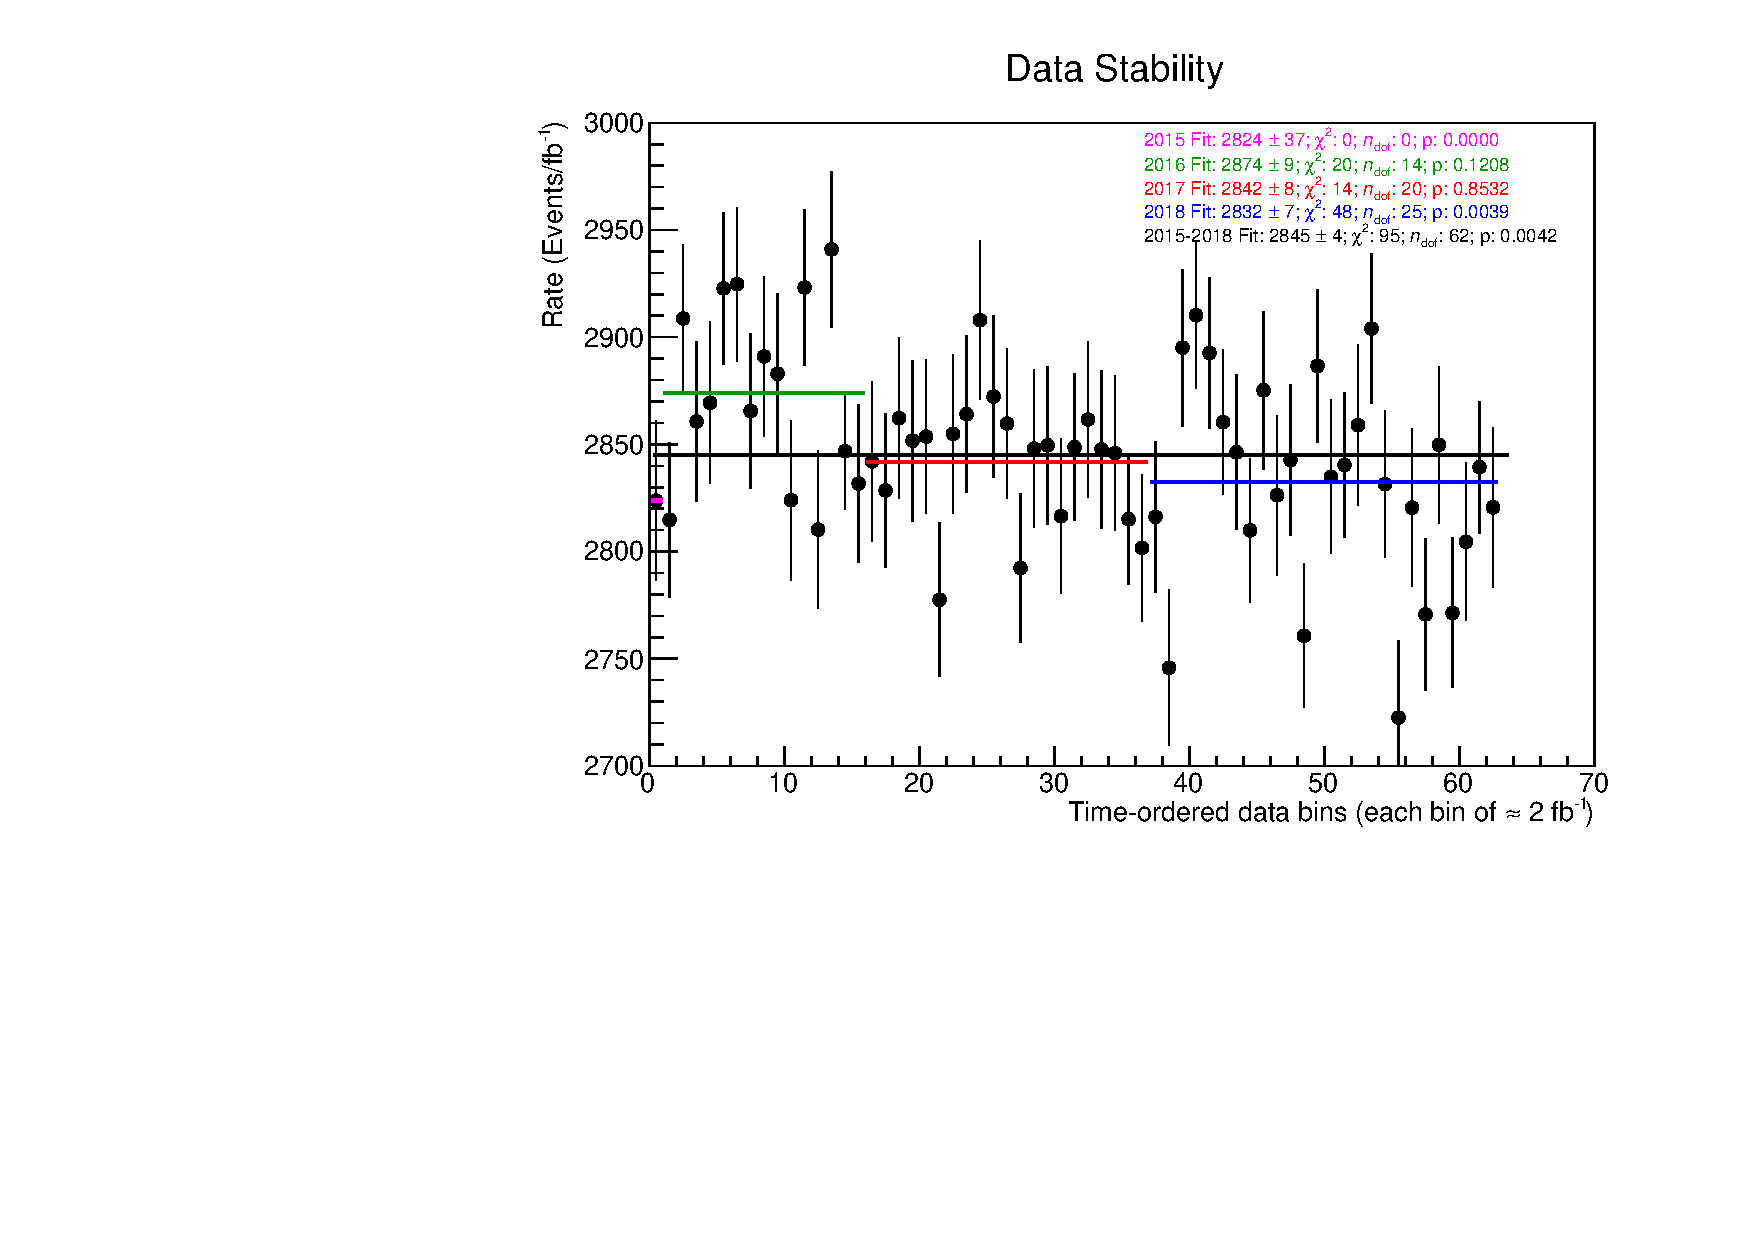
\includegraphics[width=0.75\textwidth]{figures/DataStability.pdf}
\caption{Events per fb$^{-1}$ for year 2015 to 2018, where each time-ordered data bin contains 2 fb$^{-1}$ luminosity.}
\label{fig:DataStability}
\end{figure}

\subsection{Data and Monte Carlo comparison}

Table~\ref{tab:CFComp} compares the event yields after applying the analysis cuts with data and the 2 MC samples for each year, and table~\ref{tab:RelCF} shows a relative comparison between the cuts.

\begin{table}[h!]
    \centering
    \begin{tabular}{l|l|l|l|l|l|l}
    \hline\hline
    \textbf{Sample} & \multicolumn{6}{c}{\textbf{Cuts}} \\ \hline
     & None & DQ & Trigger & Dilepton & $p_{\text{T},\ell\ell}$ & $p_{\text{T},\ell\ell}$ \\
     &  &  &  &  & $>165~\GeV$ & $>200~\GeV$ \\ \hline\hline
    Data 2015-2016 & 475.7M & 462.5M & 72.89M & 20.27M & 103.5k & 54.92k \\ \hline
    Powheg Pythia 8 MC16a & 70.63M & 70.28M & 41.27M & 20.11M & 79.31k & 41.15k \\ \hline
    Sherpa 2.2.1 MC16a & 75.60M & 75.21M & 42.28M & 20.06M & 96.72k & 52.03k \\ \hline\hline
    Data 2017 & 282.8M & 270.5M & 84.38M & 24.15M & 124.2k & 65.87k \\ \hline
    Powheg Pythia 8 MC16d & 86.42M & 85.88M & 50.35M & 24.45M & 96.58k & 50.08k \\ \hline
    Sherpa 2.2.1 MC16d & 92.50M & 91.90M & 51.59M & 24.41M & 118.3k & 63.30k \\ \hline\hline
    Data 2018 & 357.0M & 348.7M & 116.8M & 35.99M & 163.4k & 86.35k \\ \hline
    Powheg Pythia 8 MC16e & 114.0M & 113.3M & 67.22M & 32.46M & 128.2k & 66.56k \\ \hline
    Sherpa 2.2.1 MC16e & 122.0M & 121.3M & 68.93M & 36.41M & 155.9k & 83.23k \\ \hline\hline
    \end{tabular}
    \caption{Number of events remaining after each cut applied during the analysis. Data Quality (DQ) includes the GRL and event cleaning criteria.
    Dilepton includes the checks for 2 oppositely charged muons which pass TTVA and trigger matching requirements, as well as the $m_{\ell\ell}$ cut.
    Differences between MC and data are expected up to the dilepton cut as data contains QCD background while the MC samples do not.}
    \label{tab:CFComp}
\end{table}

\begin{table}[h!]
  \centering
  \begin{tabular}{l|l|l|l|l|l}
  \hline\hline
  \textbf{Sample} & \multicolumn{5}{c}{\textbf{Cuts}} \\ \hline
    & DQ & Trigger & Dilepton & $p_{\text{T},\ell\ell}$ & $p_{\text{T},\ell\ell}$ \\
    &  &  &  & $>165~\GeV$ & $>200~\GeV$ \\ \hline\hline
   Data 2015-2016 & -2.46\% & -84.24\% & -72.20\% & -99.49\% & -46.93\% \\ \hline
   Powheg Pythia 8 MC16a & -0.50\% & -41.27\% & -51.27\% & -99.61\% & -48.11\% \\ \hline
   Sherpa 2.2.1 MC16a & -0.50\% & -43.78\% & -52.56\% & -99.52\% & -46.21\% \\ \hline\hline
   Data 2017 & -4.35\% & -68.61\% & -71.38\% & -99.49\% & -46.93\% \\ \hline
   Powheg Pythia 8 MC16d & -0.63\% & -41.37\% & -51.45\% & -99.60\% & -48.15\% \\ \hline
   Sherpa 2.2.1 MC16d & -0.64\% & -43.87\% & -52.68\% & -99.52\% & -46.51\% \\ \hline\hline
   Data 2018 & -2.30\% & -66.50\% & -72.88\% & -99.48\% & -47.04\% \\ \hline
   Powheg Pythia 8 MC16e & -0.60\% & -40.69\% & -51.70\% & -99.61\% & -48.97\% \\ \hline
   Sherpa 2.2.1 MC16e & -0.60\% & -43.17\% & -52.95\% & -99.52\% & -46.63\% \\ \hline\hline
   \end{tabular}
   \caption{The relative number of events rejected after each cut compared to the previous cut}
   \label{tab:RelCF}
\end{table}

Figure~\ref{fig:MuActual} shows the actual interactions per bunch crossing $\mu$ for the individual data periods, as well as the full Run 2 dataset.
Figure~\ref{fig:pTmll} gives the $\pt$ and $m$ distributions for the dilepton system, and figure~\ref{fig:pTetamus} gives the $\pt$ and $\eta$ distributions for both the leading and sub-leading muon.
The $\pt$ and $y$ distributions for the leading and sub-leading track jet are shown in figure~\ref{fig:pTyjets}, and figure~\ref{fig:jetsubstructure} and~\ref{fig:ntrackinjets} show some
selected jet substructure variables and the number of constituents, respectively. Finally, the properties of the tracks used for the analysis are shown in figure~\ref{fig:trackInfo}.

Figure~\ref{fig:EventDisplay} shows an example event display for an event which passes all analysis cuts.

\begin{figure}[h!]
  \centering
  \includegraphics[page=5,width=0.45\textwidth]{figures/ZjetOmnifoldMCDataComp.pdf}
  \includegraphics[page=6,width=0.45\textwidth]{figures/ZjetOmnifoldMCDataComp.pdf} \\
  \includegraphics[page=7,width=0.45\textwidth]{figures/ZjetOmnifoldMCDataComp.pdf}
  \includegraphics[page=8,width=0.45\textwidth]{figures/ZjetOmnifoldMCDataComp.pdf}
  \caption{The actual interactions per bunch crossing, $\mu$, for 2015-2016 data (top left), 2017 data (top right), 2018 data (bottom left), and the full Run-2 dataset (bottom right)}
  \label{fig:MuActual}
\end{figure}

\begin{figure}[h!]
  \centering
  \includegraphics[page=12,width=0.45\textwidth]{figures/ZjetOmnifoldMCDataComp.pdf}
  \includegraphics[page=16,width=0.45\textwidth]{figures/ZjetOmnifoldMCDataComp.pdf}
  \caption{Distributions for the $\pt$ and $m$ of the dilepton system. Due to the high $\pt$ phase space, it is expected that the MC simulation will underpredict the data.}
  \label{fig:pTmll}
\end{figure}

\begin{figure}[h!]
  \centering
  \subfloat[Leading muon]{\includegraphics[page=24,width=0.45\textwidth]{figures/ZjetOmnifoldMCDataComp.pdf}\includegraphics[page=32,width=0.45\textwidth]{figures/ZjetOmnifoldMCDataComp.pdf}} \\
  \subfloat[Sub-leading muon]{\includegraphics[page=28,width=0.45\textwidth]{figures/ZjetOmnifoldMCDataComp.pdf}\includegraphics[page=36,width=0.45\textwidth]{figures/ZjetOmnifoldMCDataComp.pdf}}
  \caption{The $\pt$ and $\eta$ distributions for the (a) leading and (b) the sub-leading muon}
  \label{fig:pTetamus}
\end{figure}

\begin{figure}[h!]
  \centering
  \subfloat[Leading track jet]{\includegraphics[page=72,width=0.45\textwidth]{figures/ZjetOmnifoldMCDataComp.pdf}\includegraphics[page=76,width=0.45\textwidth]{figures/ZjetOmnifoldMCDataComp.pdf}} \\
  \subfloat[Sub-leading track jet]{\includegraphics[page=88,width=0.45\textwidth]{figures/ZjetOmnifoldMCDataComp.pdf}\includegraphics[page=92,width=0.45\textwidth]{figures/ZjetOmnifoldMCDataComp.pdf}}
  \caption{The $\pt$ and $y$ distributions for the (a) leading and (b) the sub-leading jet}
  \label{fig:pTyjets}
\end{figure}

\begin{figure}[h!]
  \centering
  \includegraphics[page=84,width=0.45\textwidth]{figures/ZjetOmnifoldMCDataComp.pdf}
  \includegraphics[page=100,width=0.45\textwidth]{figures/ZjetOmnifoldMCDataComp.pdf} \\
  \includegraphics[page=104,width=0.45\textwidth]{figures/ZjetOmnifoldMCDataComp.pdf}
    \includegraphics[page=116,width=0.45\textwidth]{figures/ZjetOmnifoldMCDataComp.pdf}\\
  \includegraphics[page=108,width=0.45\textwidth]{figures/ZjetOmnifoldMCDataComp.pdf}
      \includegraphics[page=120,width=0.45\textwidth]{figures/ZjetOmnifoldMCDataComp.pdf}\\
  \includegraphics[page=112,width=0.45\textwidth]{figures/ZjetOmnifoldMCDataComp.pdf}
      \includegraphics[page=124,width=0.45\textwidth]{figures/ZjetOmnifoldMCDataComp.pdf}
  \caption{Jet substructure features for the leading (left) and subleading (right) track jets.}
  \label{fig:jetsubstructure}
\end{figure}

\begin{figure}[h!]
  \centering
  \includegraphics[page=136,width=0.45\textwidth]{figures/ZjetOmnifoldMCDataComp.pdf}
  \includegraphics[page=140,width=0.45\textwidth]{figures/ZjetOmnifoldMCDataComp.pdf} \\
  \caption{The number of constituents in the leading (left) and subleading (right) track jets.}
  \label{fig:ntrackinjets}
\end{figure}

\begin{figure}[h!]
  \centering
  \includegraphics[page=128,width=0.45\textwidth]{figures/ZjetOmnifoldMCDataComp.pdf}
  \includegraphics[page=144,width=0.45\textwidth]{figures/ZjetOmnifoldMCDataComp.pdf} \\
  \includegraphics[page=148,width=0.45\textwidth]{figures/ZjetOmnifoldMCDataComp.pdf}
  \includegraphics[page=152,width=0.45\textwidth]{figures/ZjetOmnifoldMCDataComp.pdf}
  \caption{Distributions for the number of tracks per event (top left), and the $\pt$ (top right), $\eta$ (bottom left), and $\phi$ (bottom right) for each reconstructed track}
  \label{fig:trackInfo}
\end{figure}

\begin{figure}[h!]
  \centering
  \includegraphics[page=6,width=0.45\textwidth]{figures/EventDisplays.pdf}
  \includegraphics[page=7,width=0.45\textwidth]{figures/EventDisplays.pdf} \\
  \includegraphics[page=8,width=0.45\textwidth]{figures/EventDisplays.pdf}
  \caption{An event display for an event which passes all cuts. For the reconstructed event (top left) and the particle level event (top right), the centre of the dilepton system is shown with a red X and the individual muons with a red dot.
  Track jets are shown with a blue circle, and leading jet constituents are represented with a black X while other jet constituents are shown with a purple X. The leading jet is also shown (bottom), with the reconstructed constituents represented
  by a black X, and truth charged hadrons represented by a blue circle.}
  \label{fig:EventDisplay}
\end{figure}

\clearpage
